%!TEX root = ../thesis.tex

\chapter{Data} \label{ch:data}

\nocite{*}

\newthought{In order to carry out the analysis herein,} it was necessary to gather
play-by-play data with complete lineups. To do this, I collected the relevant data
from basketball-reference.com; this site was chosen for several reasons. First, the
website makes its data freely available and is organized simply and effectively,
simplifying the scraping process. The second and more important reason the site was
chosen was because it assigns unique identifiers to each entity for which it has
data, including players, teams, seasons, coaches, and referees.  Using these unique
identifiers, it is very easy to cross-reference and join different data sources from
the site; this makes complex analyses simpler because there it eliminates guesswork
and ambiguities in data wrangling. For example, while other data sources may have
ambiguities arising from players with similar names, Basketball Reference's unique
identifiers make it easy to distinguish between, for example, Tim Hardaway Jr.
and Tim Hardaway Sr. or Isiah Thomas and Isaiah Thomas.

The data was scraped in Python using the sportsref library, an open-source Python
library for scraping sports data from the Sports Reference family of
websites
\footnote{In addition to basketball-reference.com, this family of websites
includes sports-reference.com, baseball-reference.com, and
pro-football-reference.com.}.
I am the creator and, as of this writing, the sole developer and maintainer of the
library, which was created to make sports analytics easier for those who understand
sports and basic data analysis but do not have the programming knowledge to scrape
data themselves. The library is still in the early stages of development; its
code can be found on GitHub
\footnote{github.com/mdgoldberg/sportsref}.

More specifically, the majority of the data used in this thesis was scraped from
Basketball Reference's play-by-play section it has for almost every game since the
beginning of the 2000-2001 NBA season \footnote{For example, see
www.basketball-reference.com/boxscores/pbp/201604010GSW.html}. This page gives
detailed text descriptions of each event throughout the game, but does not contain
structured data to identify, for example, whether an event is a rebound or who the
shooter is on a field goal attempt. Therefore, regular expressions were constructed
for each type of event in the dataset in order to create structured data from these
descriptions; altogether, there are about twenty different types of descriptions.

Moreover, several issues exist in the raw data that required cleaning. Perhaps the
most difficult problem with the raw data was that some events were ordered
incorrectly. Examples include rebounds being listed prior to their corresponding
missed shots and inconsistencies surrounding when substitutions and timeouts occur
during free throws; these problems were remedied by a complicated sorting scheme
within each possession. Other, slightly simpler problems included tracking which
team was on offense or defense at any given time and consolidating redundant
substutitions in which a player would sub in and immediately sub out.

Once the raw data was cleaned, additional features were added to the data. Simple
new features include keeping track of the home and away teams' points scored on each
event, so that point differential can easily be computed for any subset of events.
One very important and more complicated feature was identifying ``plays,'' a
possession-like concept for which Maymin et al advocates. In particular, the
definition of a play is identical to the definition of a possession, except that an
offensive rebound extends a possession but begins a new play. Differentiating plays
was done by labeling events that end a play with an indicator variable and computing
the cumulative sum of these variables to create a play identification number for
each event. Specifically, play-ending events include turnovers, field goal attempts
on which fouls were not committed, non-technical free throws that are not succeeded
by another free throw, and the end of each quarter or overtime period.

% TODO: discuss collecting lineup data
* Used parsed play-by-play data to determine who is in the game at any given point
    - mention issue with quarter starters

% TODO: display some data for an example (table? pweave?)

* Engineered player profile features from play-by-play data
    - go over player profile

% \begin{figure}
% 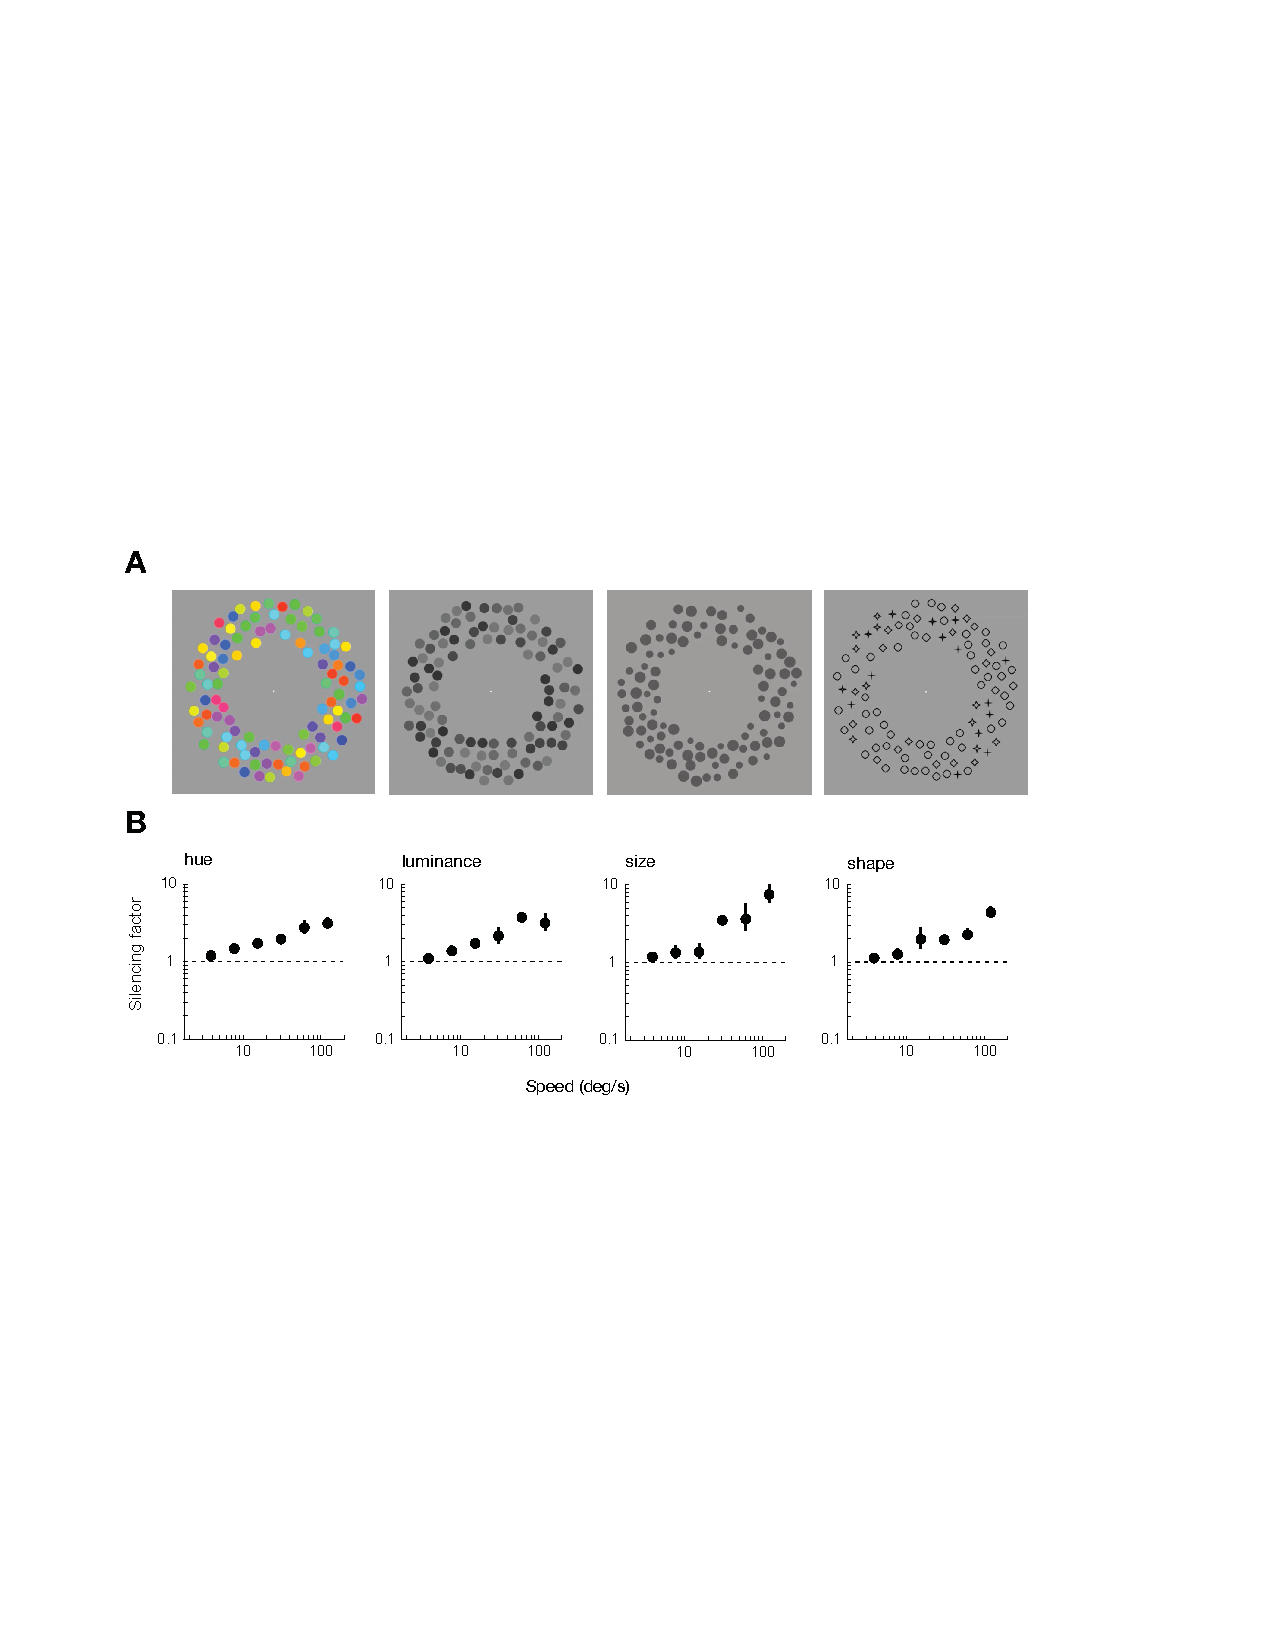
\includegraphics[width=\textwidth]{figures/fig1}
% \caption[Short figure name.]{This is a figure that floats inline and here is its caption.
% \label{fig:myInlineFigure}}
% \end{figure}

%% Requires fltpage2 package
%%
% \begin{FPfigure}
% 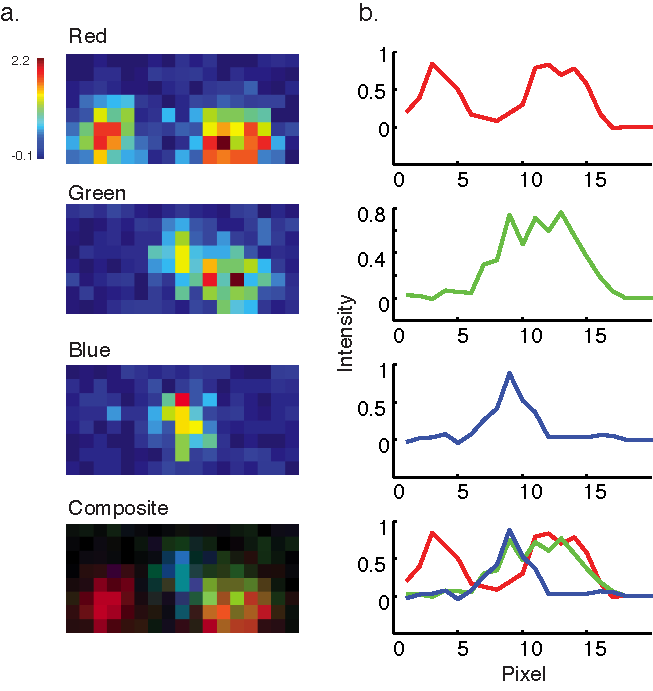
\includegraphics[width=\textwidth]{figures/fullpage}
% \caption[Short figure name.]{This is a full page figure using the FPfigure command. It takes up the whole page and the caption appears on the preceding page. Its useful for large figures. Harvard's rules about full page figures are tricky, but you don't have to worry about it because we took care of it for you. For example, the full figure is supposed to have a title in the same style as the caption but without the actual caption. The caption is supposed to appear alone on the preceding page with no other text. You do't have to worry about any of that. We have modified the fltpage package to make it work. This is a lengthy caption and it clearly would not fit on the same page as the figure. Note that you should only use the FPfigure command in instances where the figure really is too large. If the figure is small enough to fit by the caption than it does not produce the desired effect. Good luck with your thesis. I have to keep writing this to make the caption really long. LaTex is a lot of fun. You will enjoy working with it. Good luck on your post doctoral life! I am looking forward to mine. \label{fig:myFullPageFigure}}
% \end{FPfigure}
% \afterpage{\clearpage}

